% Created 2021-01-27 Wed 11:07
% Intended LaTeX compiler: pdflatex
\documentclass[11pt]{article}
\usepackage[utf8]{inputenc}
\usepackage[T1]{fontenc}
\usepackage{graphicx}
\usepackage{grffile}
\usepackage{longtable}
\usepackage{wrapfig}
\usepackage{rotating}
\usepackage[normalem]{ulem}
\usepackage{amsmath}
\usepackage{textcomp}
\usepackage{amssymb}
\usepackage{capt-of}
\usepackage{hyperref}
\author{Patryk Kaniewski}
\date{\today}
\title{}
\hypersetup{
 pdfauthor={Patryk Kaniewski},
 pdftitle={},
 pdfkeywords={},
 pdfsubject={},
 pdfcreator={Emacs 27.1 (Org mode 9.3)}, 
 pdflang={English}}
\begin{document}

\tableofcontents \clearpage\begin{center}
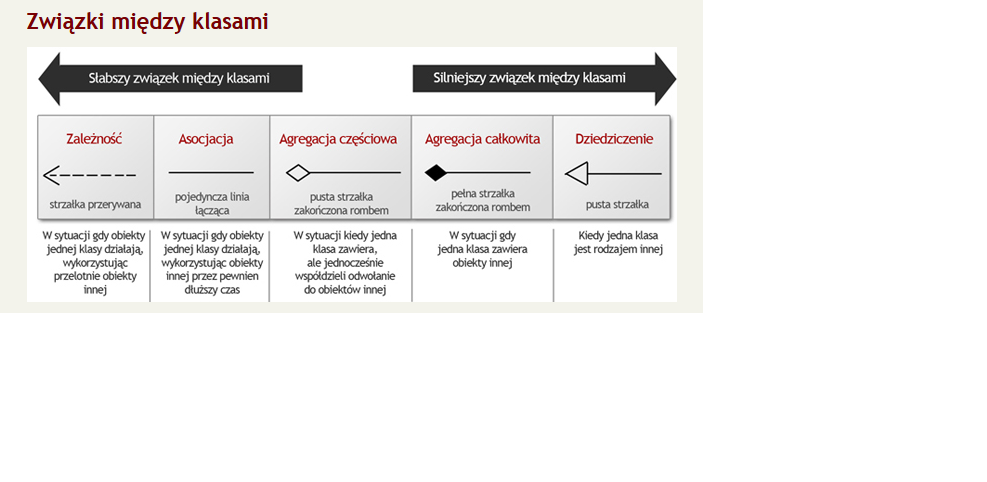
\includegraphics[width=.9\linewidth]{./zwiazki_UML.png}
\end{center}

\section{wzorce kreacyjne}
\label{sec:orga7a56ae}
\subsection{singleton}
\label{sec:org6a6d852}
\begin{center}
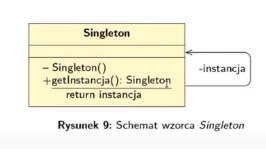
\includegraphics[width=.9\linewidth]{./singleton.png}
\end{center}
\begin{itemize}
\item zagwaratowac ze jest jeden obiekt tego typu (np. konfiguracja/stan globalny)
\end{itemize}
\subsubsection{implementacja}
\label{sec:org0403ba6}
\begin{verbatim}

class singleton {

private static singleton; //nasz obiekt
public static singleton getSingleton() //statyczna publiczna funkcja do otrzymywania tego stanu
{
	if(instancja==null)
		instancja = new Singleton();

	return singleton;
}
};

\end{verbatim}
\subsection{iterator}
\label{sec:org3baca9e}
\begin{itemize}
\item hermetyzacja iteracji
\end{itemize}
\begin{verbatim}
Iterator iterator = menuCostam.utworzIterator();
while (iterator.hasNext())
{
 pozycjaMenu pozycja = iterator.next();
}
\end{verbatim}

\section{wzorce behawioralne}
\label{sec:org5381483}
\subsection{Obserwator}
\label{sec:orgbd64461}
\begin{center}
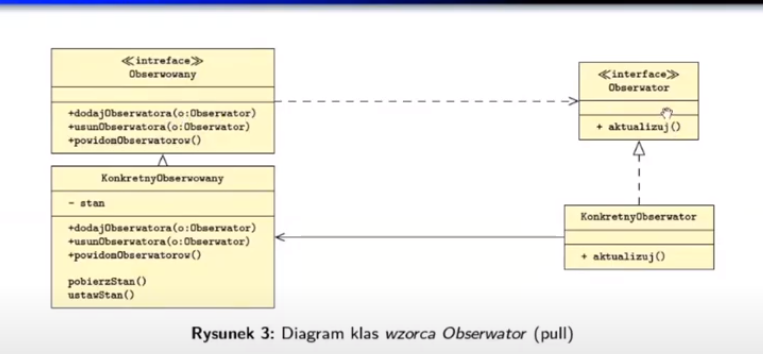
\includegraphics[width=.9\linewidth]{./obserwator.png}
\end{center}
\begin{itemize}
\item okresla zaleznosc jeden do wiele miedzy obiektami
\item gdy jeden obiekt zmienia stan wszystkie obiekty od niego zalezne sa o tym automatycznie powiadamiane i uaktualniane (np. w kalkulatorze mamy 3 klasy wypisywania ktore maja w sobie string do wypisywania, kiedy wprowadzamy nowe dzialanie wszyskie sa updatowane)
\item wydaje mi sie ze realizowany w grach -> bo trzeba updatowac stan obiektow a one musza znac stan innych
\end{itemize}
\subsubsection{kontekst}
\label{sec:org14eb0e2}
zmiana stanu jednego obiektu wymaga zmiany innych i nie wiadomo, ile obiektow trzeba zmienic
\subsubsection{problem}
\label{sec:org041c0c7}
obiekt powinien byc w stanie powiadamiac inne obiekty, nie przyjmujac zadnych zalozen co do tego, co te obiekty reprezentuja - wynikiem sa luzniejsze powiazania miedzy obiektami
\subsubsection{implementacja}
\label{sec:orgaabf340}
\url{https://refactoring.guru/design-patterns/observer}
zagwarantowanie ze przed rozeslaniem powiadomienia stan obserwowanergo jest wewnetrznie spojny


model push (obserwowany wysyla wszystkie informacje same)
model pull (obserwowany wysyla POWIADOMIENIE a kazdy inny pyta sie to czego potrzebuje z jakiejs zmiany)
\subsection{Stan}
\label{sec:org26a7210}
\begin{itemize}
\item umozliwia obiektowi zmiane zachowania, gdy zmienia sie jego stan wewnetrzny (np. ktos zmienia typ konta bankowego)
\end{itemize}
\subsubsection{kontekst}
\label{sec:org037bf63}
\begin{itemize}
\item zachowanie obiektu zalezy od jego stanu, a obiekt ten musi zmieniac swoje zachowanie w czasie wykonywania programu w zaleznosci od stanu
\item operacje zawieraja duze, wieloczesciowe instrukcje warunkowe ktore zaleza od stanu obiektu - wzorzec State przenosi kazde rozgalezienie do specjalnej klasy z inna implementacja np. pobierz podatek
\end{itemize}
\subsubsection{problem}
\label{sec:org0787654}
chemy umozliwic obiektowi zmiane zachowania w momencie zmiany wewnetrzengo stanu obiektu hermetyzujac stan w postaci klasy
\subsubsection{implementacja}
\label{sec:orgdbef42e}
\begin{center}
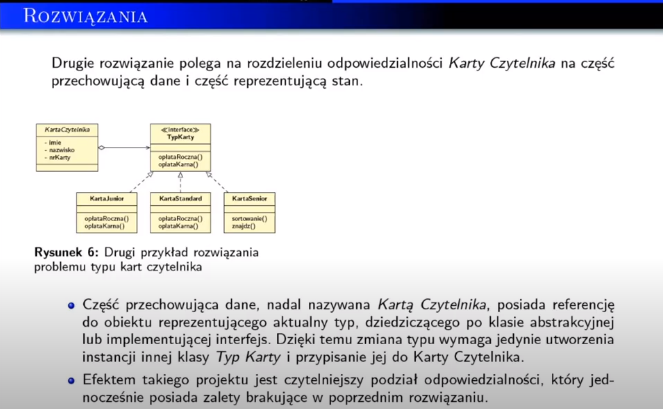
\includegraphics[width=.9\linewidth]{./stan.png}
\end{center}
\subsection{strategia}
\label{sec:orgedad967}
\begin{itemize}
\item 
\end{itemize}
\section{wzorce strukturalne}
\label{sec:org13c94a5}
\subsection{kompozyt}
\label{sec:orgb84edc7}
\begin{center}
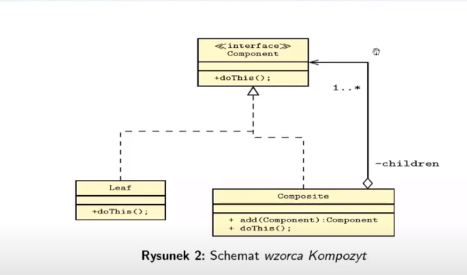
\includegraphics[width=.9\linewidth]{./kompozyt.png}
\end{center}
TLDR: Drzewko w ktorym lisc zawiera siebie + liste dzieci

\begin{itemize}
\item zadaniem jest laczenie obiektow w struktura tak, ze reprezentuja hierarchie czesci-calosci, unifikujac dostep do kolekcji jak i pojedynczego obiektu.
\item + umozliwa to klientom jednolite traktowanie pojedynczych obiektow i rowniez ich kompozycji
\end{itemize}

\subsubsection{kontekst}
\label{sec:org927fe0d}
chcemy przedstawic hierarchie obiektow czesc-calosc Hierarchia obiektow ma wspolna klase bazowa (abstrakcyjną)
\subsubsection{problem}
\label{sec:org9375bc7}
chcemy, aby klienci mogli ignorowac roznice miedzy zlozeniami obiektow a pojedynczymi obiektami - klienci beda wtedy jednakowo traktowac wszyskie obiekty wystepujace w strukturze
\end{document}
